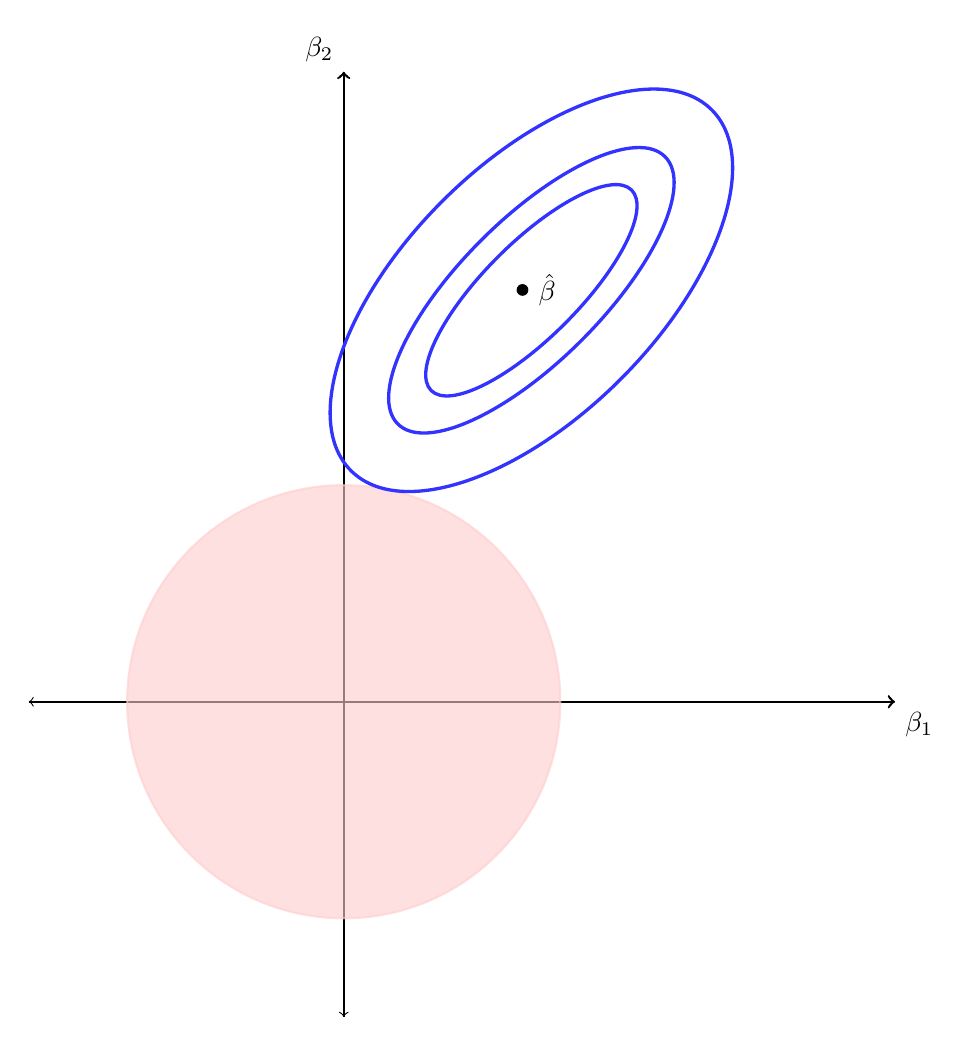
\begin{tikzpicture}
\draw[<->] (-4,0) -- (7,0) coordinate (x axis);
\draw[<->] (0,-4.0) -- (0,8.0) coordinate (y axis);
\draw[thick,->] (-4,0) -- (7,0) node[anchor=north west] {$\beta_1$};
\draw[thick,->] (0,-4) -- (0,8) node[anchor=south east] {$\beta_2$};

\draw[red!20, thick, fill, opacity=0.6] (0,0) circle (2.75cm);

\draw[very thick, blue!80, rotate=45] (5.38,2.01) ellipse (3.24cm and 1.6cm);
\draw[very thick, blue!80, rotate=45] (5.38,2.01) ellipse (2.4cm and 0.9cm);
\draw[very thick, blue!80, rotate=45] (5.38,2.01) ellipse (1.8cm and 0.60cm);

\node at (2.27,5.23)[circle,fill,inner sep=1.5pt, label=right:$\hat{\beta}$]{};
\end{tikzpicture}

